\chapter{Experiments}
\label{Experiments}


\section*{Model select}
Approximately a decade has passed since Goodfellow introduced Generative Adversarial Networks (GANs), 
during which numerous variants of GAN models have been developed. For the purpose of this study, 
I have selected seven distinct GAN models for examination and minimal implementation: Standard GANs, 
Conditional GANs, Auxiliary Classifier GANs, Cycle GANs, Domain Transfer Network GANs, Coupled GANs, 
and Style GANs. The primary criterion for selection is training time, with only one model chosen for 
further in-depth analysis. Due to the extensive training time required, I ultimately selected Standard GANs for detailed study.


\section*{Model Structure}

In this step, I compared two types of standard GANs. The first model utilized dense layers, 
while the second model employed convolutional layers. The structure of the generator and discriminator 
was modified accordingly, while all other hyperparameters were kept constant. Both models 
were trained on the MNIST dataset for 1000 epochs. Upon comparing the generated images, 
it was observed that the GAN with the convolutional neural network (CNN) architecture 
outperformed the one with the dense layer architecture in terms of image quality.

\begin{figure}[H]
    \centering
    \begin{subfigure}[b]{0.45\linewidth}
        \centering
        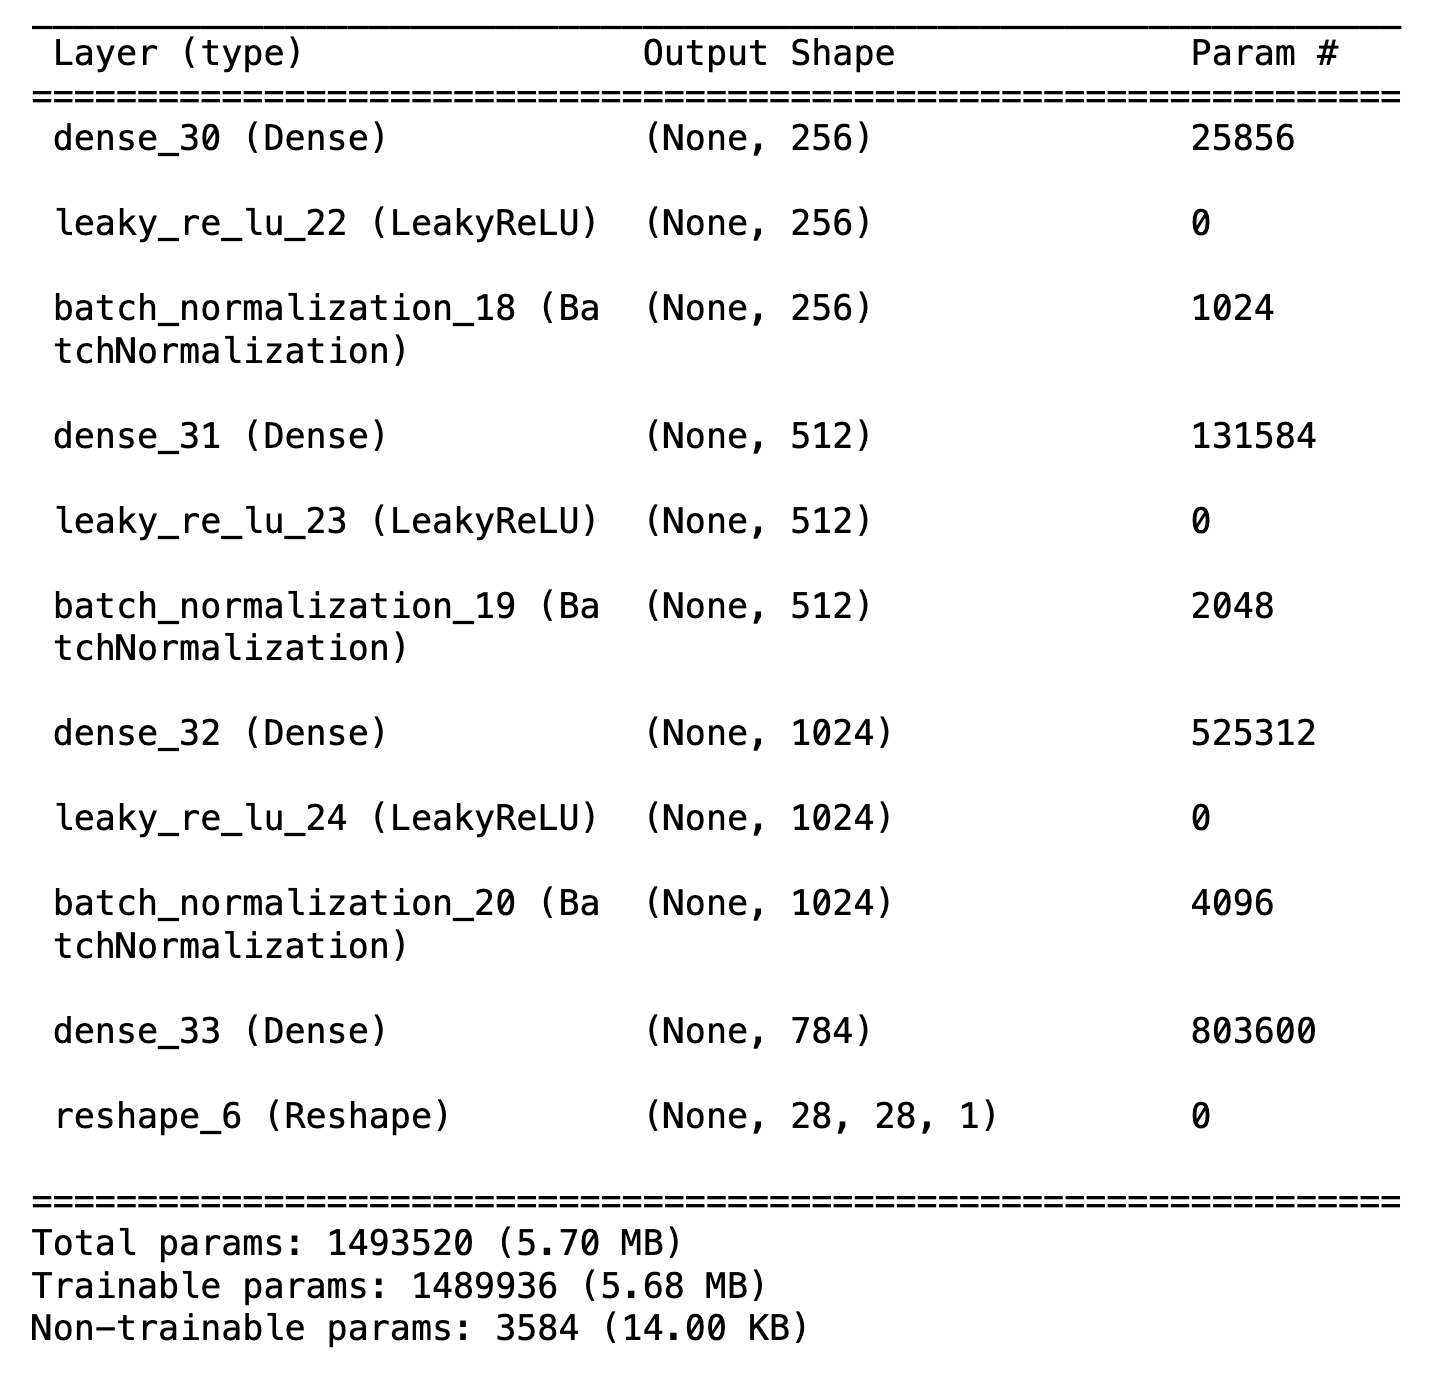
\includegraphics[width=\linewidth]{./Images/generator_dense.jpg}
        \caption{Generator with dense layer}
        \label{fig:Dense}
    \end{subfigure}
    \hspace{0.05\linewidth}
    \begin{subfigure}[b]{0.45\linewidth}
        \centering
        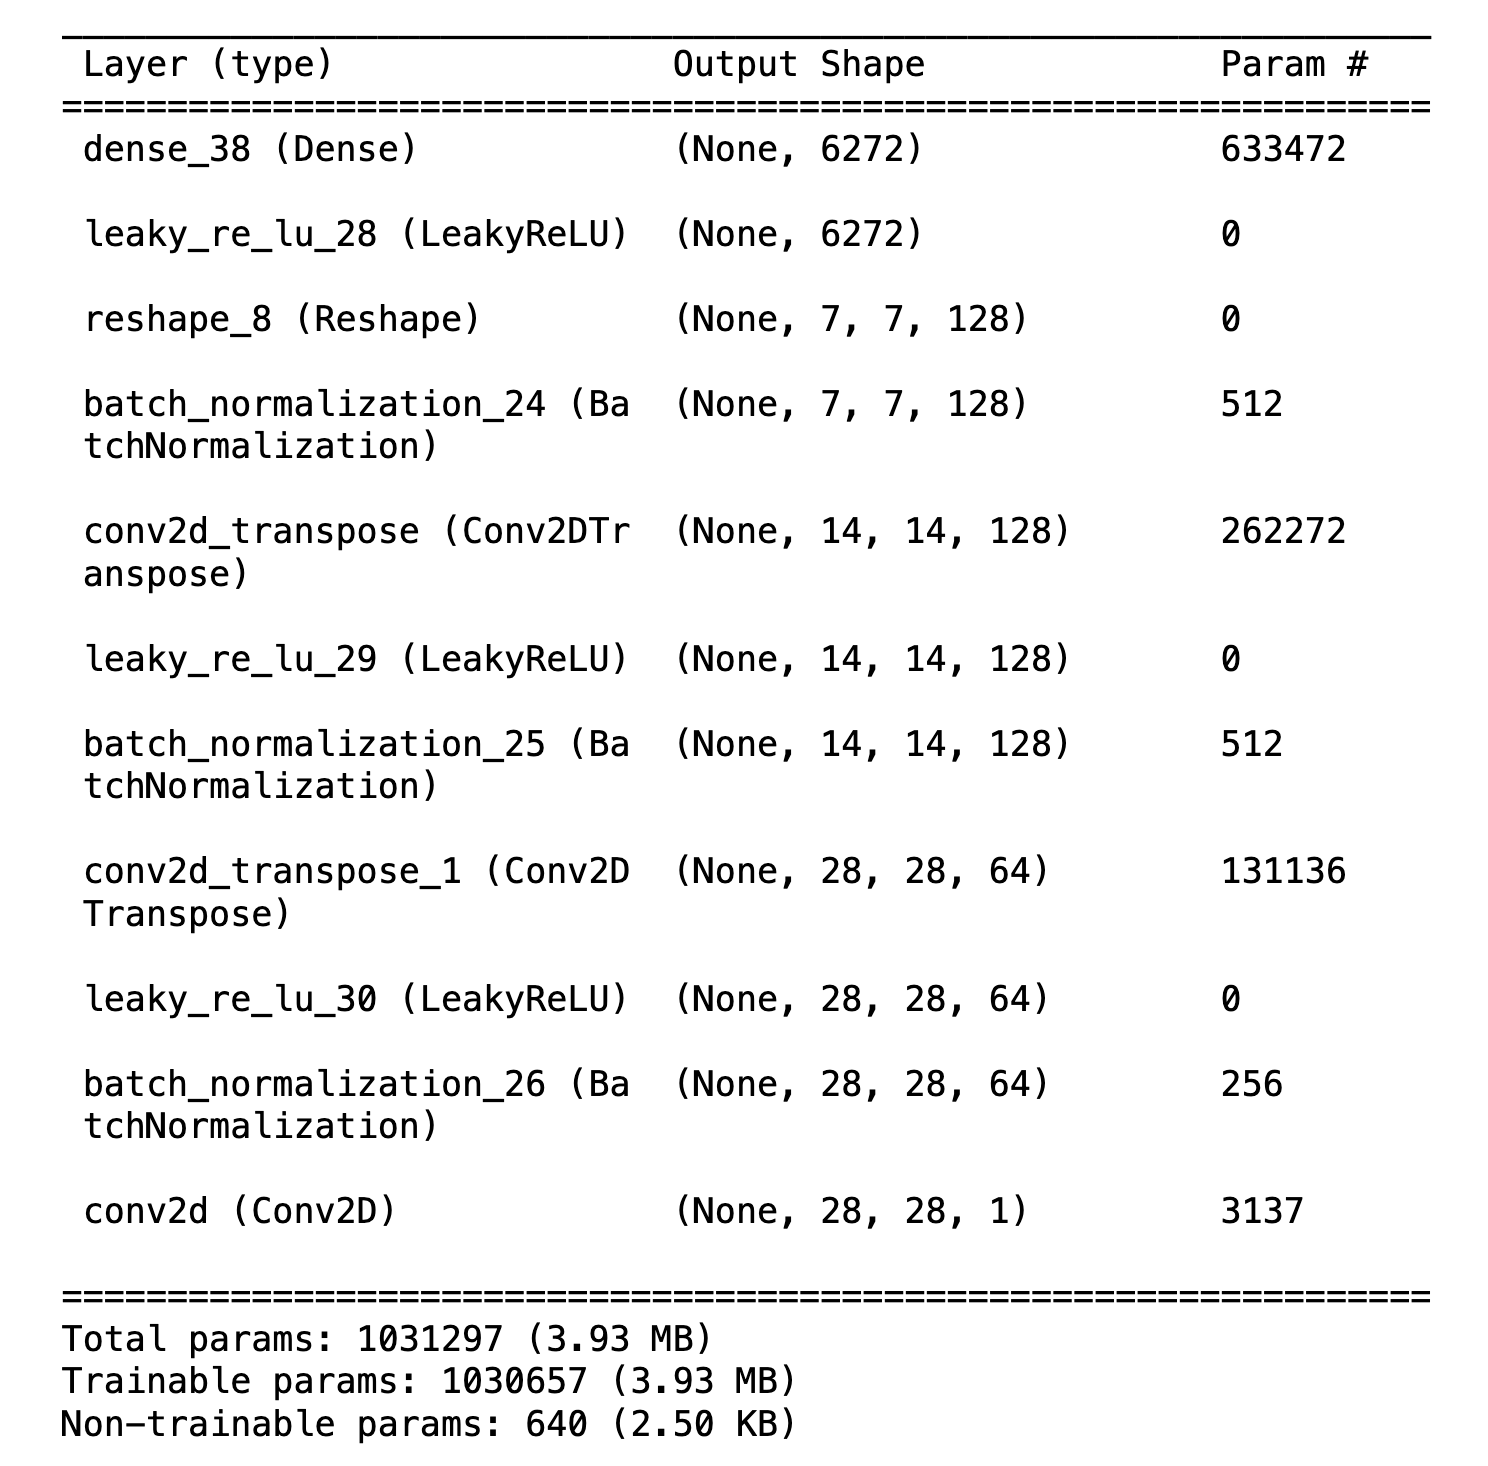
\includegraphics[width=\linewidth]{./Images/generator_cnn.jpg}
        \caption{Generator with convelution layer}
        \label{fig:Conv2D Transpose}
    \end{subfigure}
    \caption{The structure for generator}
    \label{fig:combined}
\end{figure}


\begin{figure}[H]
    \centering
    \begin{subfigure}[b]{0.45\linewidth}
        \centering
        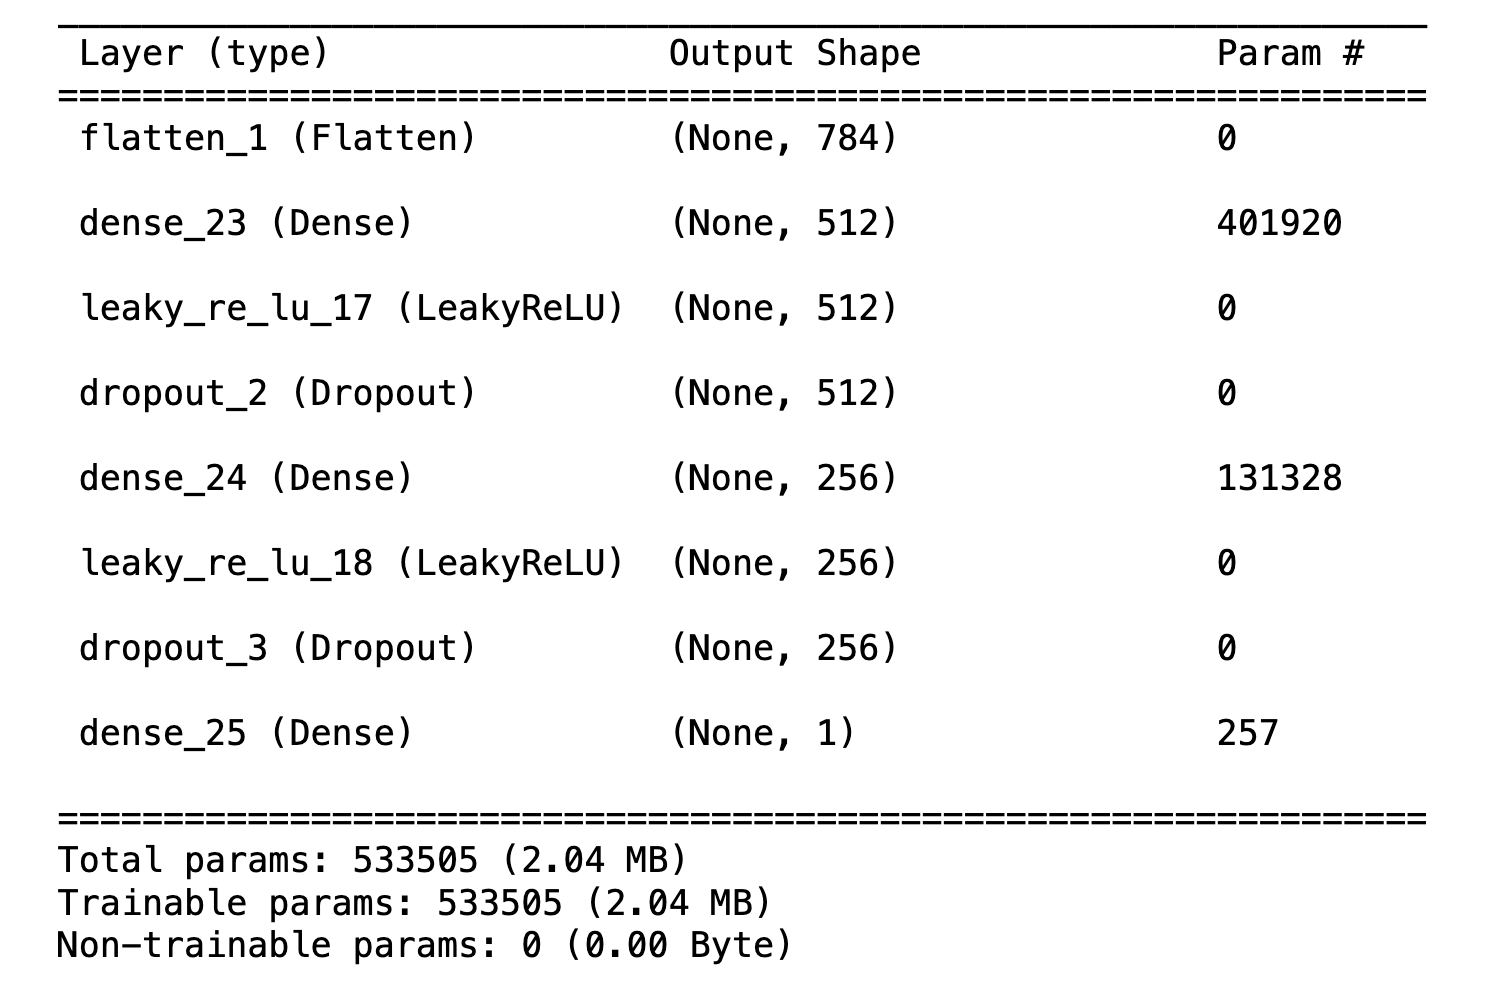
\includegraphics[width=\linewidth]{./Images/discriminator_dense.jpg}
        \caption{Discriminator with dense layer}
        \label{fig:Dense}
    \end{subfigure}
    \hspace{0.05\linewidth}
    \begin{subfigure}[b]{0.45\linewidth}
        \centering
        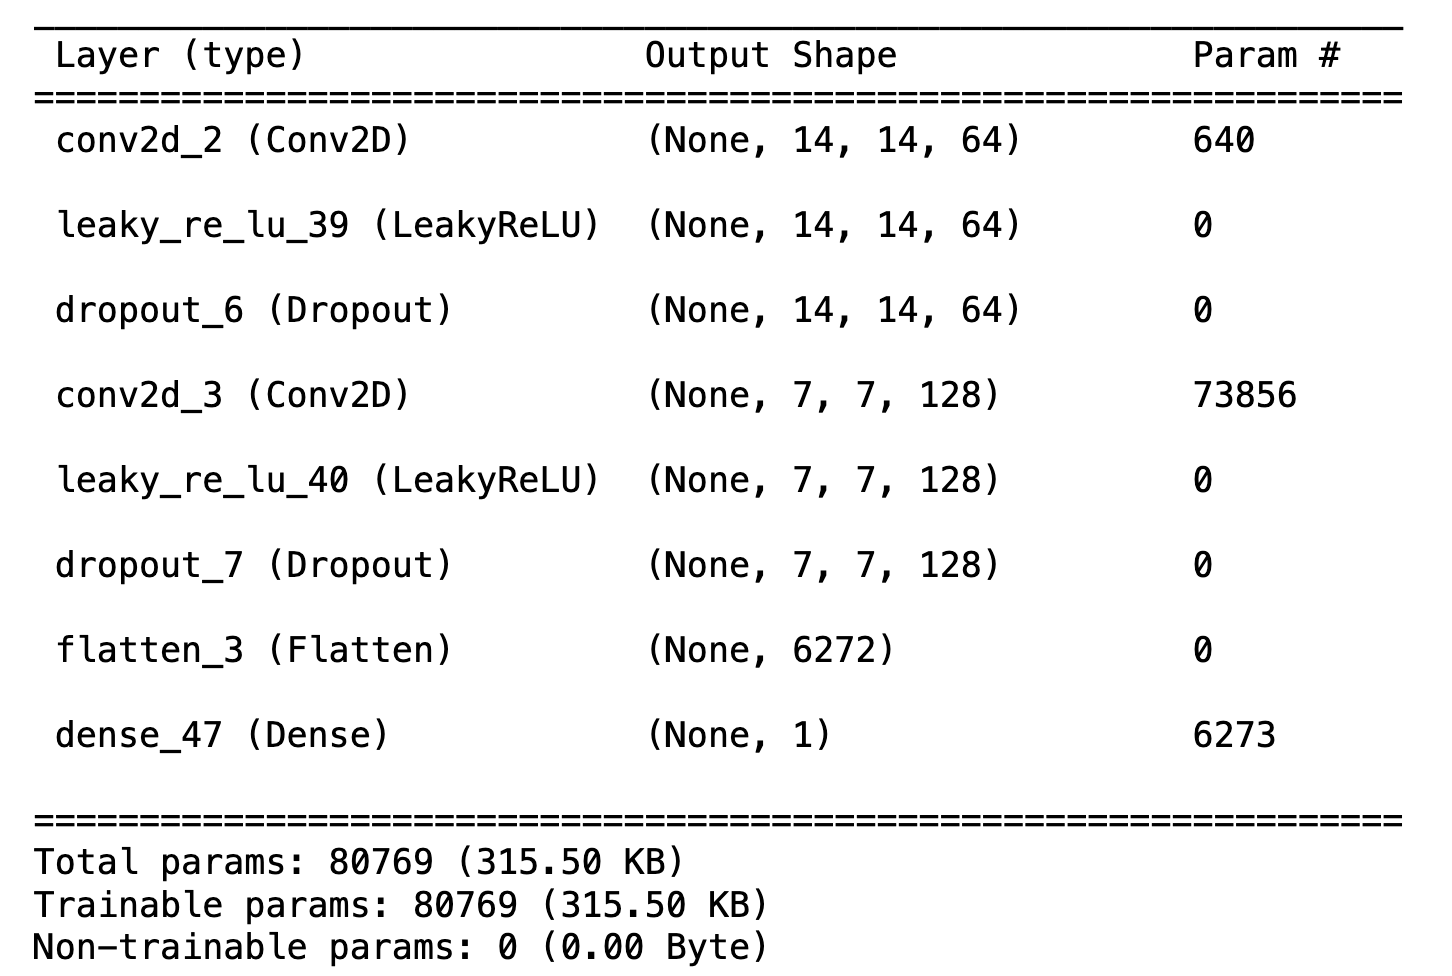
\includegraphics[width=\linewidth]{./Images/discriminator_cnn.jpg}
        \caption{Discriminator with convelution layer}
        \label{fig:Conv2D Transpose}
    \end{subfigure}
    \caption{The Structure For Discriminator}
    \label{fig:combined}
\end{figure}


\begin{figure}[H]
    \centering
    \begin{subfigure}[b]{\linewidth}
        \centering
        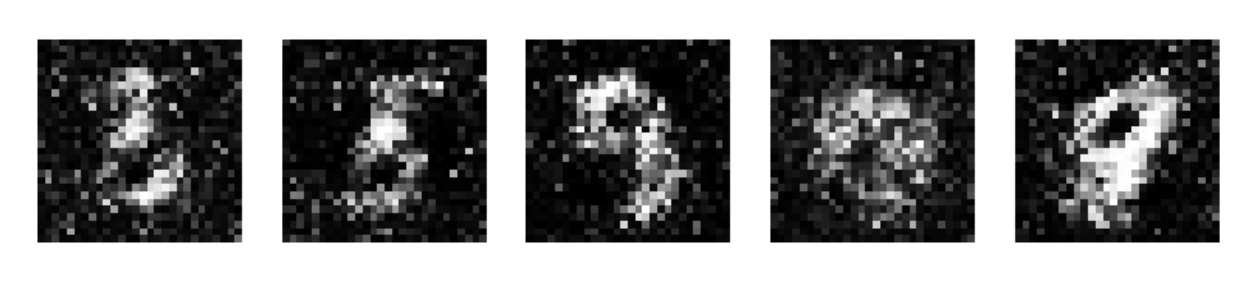
\includegraphics[width=0.7\linewidth]{./Images/generate_image_by_dense_layer.jpg}
        \caption{Images generate by dense layer}
        \label{fig:Dense}
    \end{subfigure}
    \vspace{0.05\linewidth} 
    \begin{subfigure}[b]{\linewidth}
        \centering
        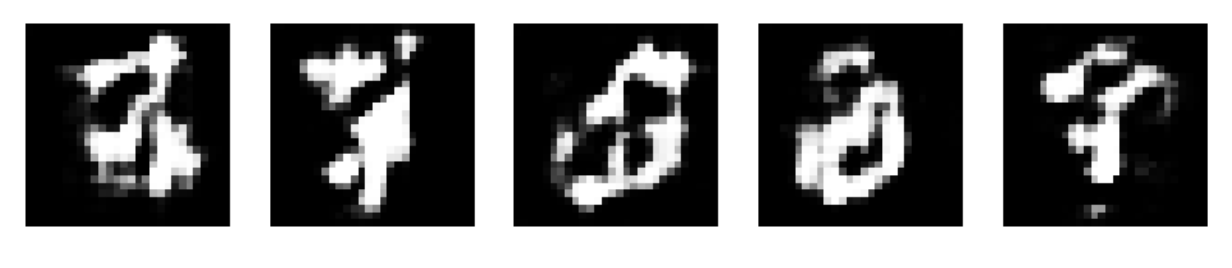
\includegraphics[width=0.7\linewidth]{./Images/generate_image_by_Convelution_layer.jpg}
        \caption{Images generate by convelution layer}
        \label{fig:Conv2DTranspose}
    \end{subfigure}
    \caption{Model performance }
    \label{fig:combined}
\end{figure}
